\documentclass{article}
\usepackage{fullpage}
\usepackage{enumerate}
\usepackage{amsmath}
\usepackage{tikz}
\usepackage{color, colortbl}

\title{CS181 Assignment 5---Markov Decision Processes and Reinforcement Learning}
\author{Lucas Freitas and Angela Li}

\begin{document}
\maketitle
    
    \begin{enumerate}
        \item
            \begin{enumerate}[(a)]
                \item We have a probability distribution $P(\text{points } | \text{ target})$ and a utility function $U(\text{points, score})$. The expected utility of aiming for a target $t$ is:

                $$\sum_{k \in K} P(\text{k} | \text{t}) \; U(\text{k, S})$$

                Where $K$ is the set of possible points scored after one throw, and $S$ is the current score. To determine the optimal action, we use the maximum expected utility principle:

                $$\underset{t \in T}{\operatorname{argmax}} \sum_{k \in K} P(\text{k} | \text{t}) \; U(\text{k, S})$$

                Where T is the set of possible targets we can aim for.

                \item This utility function works fairly well for paring down the score in a relatively small number of dart throws*, but only until it reaches the point where it is possible to win in one throw. At that point, it makes decisions poorly in that it values a non-winning throw as nearly as good as a winning throw. \\

                For example, if the current score was 20, a throw resulting in a 20-point gain would end the game (and thus should be valued extremely highly). However, a throw resulting in a 19-point gain (which requires, at the very least, one more throw to win the game) would be valued at only 5\% less utility than a winning throw. So the proposed utility function is not conducive to good decision-making in states where it is possible to win in one move---in those cases, the winning move should be valued significantly more highly. \\

                *Even a quick paring-down of the score, however, is not always desirable. Consider that there are probably significantly many more ways to score 10 points in a throw than there are ways to score 1 point in a throw. However, if the current score was 20, the utility function would reward a score of 19 higher than a score of 10, even though both point values require at the very least one more dart throw to win; a throw of 10 shoul, however, be rewarded more because it creates more opportunity for a winning throw (of 10 points) than a throw of 19 (which requires a winning throw of 1 point).
            \end{enumerate}
        \item
            \begin{enumerate}[(a)]
                \item In our MDP model, the states are the possible scores in the game (so every integer in the range [0, \texttt{START\_SCORE}] is a state), and the actions are the possible areas (ring and wedge) that the dart player can aim for in any given turn. \\

                Therefore \texttt{get\_states()} should return \texttt{range(throw.START\_SCORE + 1)}.
                \item The reward function should not depend on the action $a$ - it should only take into account if the user has won ($s==0$) or not yet.  Thus, we can write the function as \texttt{return 1 if s == 0 else 0}. The problem about this reward function is that it doesn't show our preference of winning earlier than late.\\
                
               That is why the discount factor is important - we should use it to show that bias for earlier wins. If the discount factor was $1$, then we would still not be able to add that preference (we would still not care if we won early or late), and if the discount factor was $0$, that would mean that we don't care about winning later at all, which is not good, since we will definitely need future actions in order to win eventually. Thus, we should have a discount factor between $0$ and $1$, closer to $0$ in order to show the preference for winning early.
                 \item Implementation included in appendix.
                
                \item There is no guarantee that the darts game can be won in a certain number of steps, so it doesn't make sense to impose an arbitrary finite horizon on the game---after all, the optimal policy should place primary importance on being able to get to a score of 0, and secondary importance on accomplishing that score in as few steps as possible.
                \item Running experiments for the small game, it seems that the optimal policy resulting from value iteration focuses on trying to hit an area that is going to make the user win with that throw. For instance, the program always starts aiming at edge $3$, ring $3$ at first, which would give a score of $9$ and an instantaneous win. The same happens for scores in the range $[1,6]$ - for a given score $k$ in that range, the program aims at an area that gives a score of $k$. For $7$ and $8$, on the other hand, the program aims at $2$ and $3$ respectively, which makes sense, since hitting an area and getting exactly $7$ or $8$ is not very likely (actually not even possible for $7$). Thus, the program first reduces the score and then tries to win in the next hit.
                
                \item The table below shows the program policy for values of $\gamma$ from $0$ to $1$. Each row $k$ for a given $\gamma$ has the value of the area that is aimed at when the score in the game is $k$ and the discount factor is $\gamma$.
                
\begin{center} \begin{tabular}[h]{|c|c|c|c|c|c|c|c|c|c|c|c|} \hline
\rowcolor{black}
\textcolor{white}{$\gamma/k$} & \textcolor{white}{$0.0$} & \textcolor{white}{$0.1$} &   \textcolor{white}{$0.2$} &  \textcolor{white}{$0.3$} &  \textcolor{white}{$0.4$} &  \textcolor{white}{$0.5$} &  \textcolor{white}{$0.6$} &  \textcolor{white}{$0.7$} &  \textcolor{white}{$0.8$} &  \textcolor{white}{$0.9$} &  \textcolor{white}{$1.0$}\\ \hline
$1$ & 6 & 1 & 1 & 1 & 1 & 1 & 1 & 1 & 1 & 1 & 1 \\
$2$ & 6 & 2 & 2 & 2 & 2 & 2 & 2 & 2 & 2 & 2 & 2 \\
$3$ & 6 & 3 & 3 & 3 & 3 & 3 & 3 & 3 & 3 & 3 & 3 \\
$4$ & 6 & 4 & 4 & 4 & 4 & 4 & 4 & 4 & 4 & 4 & 4 \\
$5$ & 6 & 5 & 5 & 5 & 5 & 5 & 5 & 5 & 5 & 5 & 5 \\
$6$ & 6 & 6 & 6 & 6 & 6 & 6 & 6 & 6 & 6 & 6 & 6 \\
$7$ & 6 & 2 & 2 & 2 & 2 & 2 & 2 & 2 & 2 & 1 & 1 \\
$8$ & 6 & 3 & 3 & 3 & 3 & 3 & 3 & 3 & 3 & 1 & 1 \\
$9$ & 6 & 9 & 9 & 9 & 9 & 9 & 9 & 9 & 9 & 9 & 9 \\ \hline
\end{tabular} \end{center}

From the table, we can firstly see that for $\gamma=0$ the are that is aimed at is always the same (area that gives score of $6$). That is not surprising, since a discount factor of zero would mean that we are not looking into the implications of our actions at all, so it doesn't matter what score we currently have, our strategy will always be there same.\\

Secondly, we can see that the strategy for $k=1$ to $6$ or $k=9$ and $\gamma>0$ is to always aim at an area that gives the same score as $k$. The actual wedge and ring targeted actually changes for some $\gamma$ (for $2$, for instance, it changes from wedge $2$, ring $4$ to wedge $1$, ring $5$ for $\gamma\ge0.9$).\\

Finally, we see that for $\gamma=0.9$ or $\gamma=1.0$, we do have a change in strategy,  aiming to $1$ instead of $2$ or $3$. That indicates that since $\gamma$ is getting higher, we care less and less about how long the game lasts, and the program is just aiming on finishing the game instead of finishing it fast.
            \end{enumerate}        
        \item
            \begin{enumerate}[(a)]
                \item We converge during policy iteration if $\pi_{i+1}(s) = \pi_{i}$ for every state $s$; that is, 

                $$\forall s \; V^{\pi_k}(s) = \underset{a}{\operatorname{argmax}} \sum_{s'} P(s' | s, a) [R(s, a) + \gamma V_j^{\pi_k}(s')]$$

                Since this satisfies the Bellman equation, we know that it is tha value of optimal stationary policy.
                \item If $\pi^{(1)}$ is the policy before a policy iteration phase and $\pi^{(1)}$ is the policy after, then by definition: $$\pi^{(2)}(s) = \underset{a}{\operatorname{argmax}} \; Q^{\pi^{(1)}}(s, a)$$
                
               From that, we can write that:
               
               $$Q^{\pi^{(1)}}(s, \pi^{(2)}(s))\geq V^{\pi^{(1)}}(s)$$
 If we expand $Q$, however, we will get another expression with $V^{\pi}(s_{t+1})$, and if we keep going, we will get to a point in which we get $V^{\pi^{(2)}}(s)$, which proves that:
 
 $$V^{\pi^{(e)}}(s) \geq V^{\pi^{(1)}}(s)$$  
                \item Since there are a finite number of states and actions, there are also only a finite number of stationary policies. With every step of policy iteration, we will produce either an unchanged policy or a policy that is a strict improvement over the previous. If the policy is unchanged, then we terminate---producing an optimal policy as proven in part (a). If the policy is a strict improvement, we continue; however, since there are only a finite number of policies, we must eventually reach the optimal one as less-optimal policies are disregarded.
            \end{enumerate}        
        \item
            \begin{enumerate}[(a)]
                \item 
                \begin{enumerate}[1.]
                	\item
			 For \texttt{ex\_strategy\_one}, we decided to use a very simple strategy: explore or exploit with $50\%$ probability each. That can we written simply as \texttt{return random.choice([0, 1])}. 
		\item
			 For \texttt{ex\_strategy\_two}, we decided to use the \texttt{num\_iterations} as an argument for the function, and to decrease the probability of exploration as \texttt{num\_iterations} increases. Our function was thus: \texttt{return random.random() < 1./(2 + 0.1 * num\_iterations)}\\
		  \end{enumerate}	 
			 Running the program for \texttt{EPOCH\_SIZE} from $10$ to $200$ and \texttt{num\_games=100}, for each of the two strategies, we get the performances shown in the graphs below:
			 \begin{center}
			 	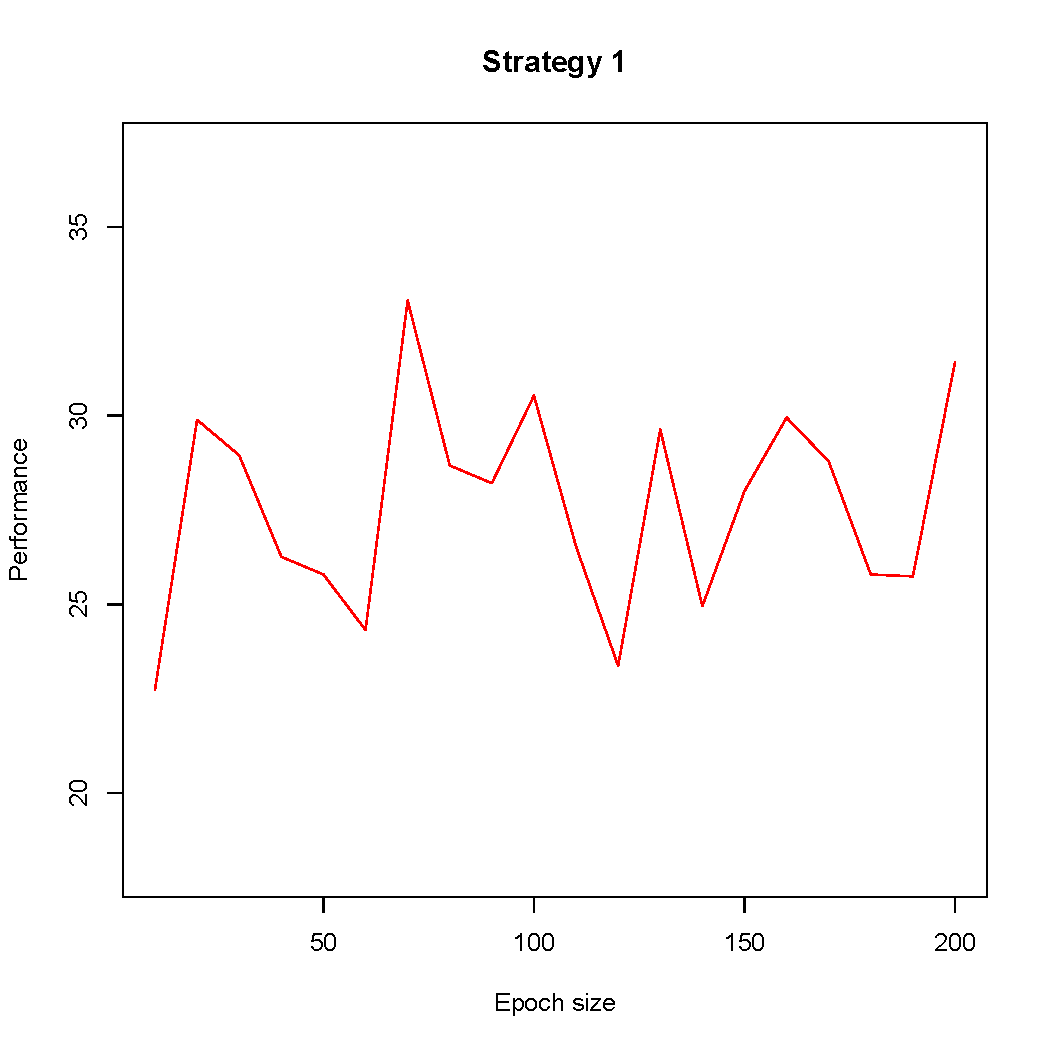
\includegraphics[width=0.4\textwidth]{graph1} 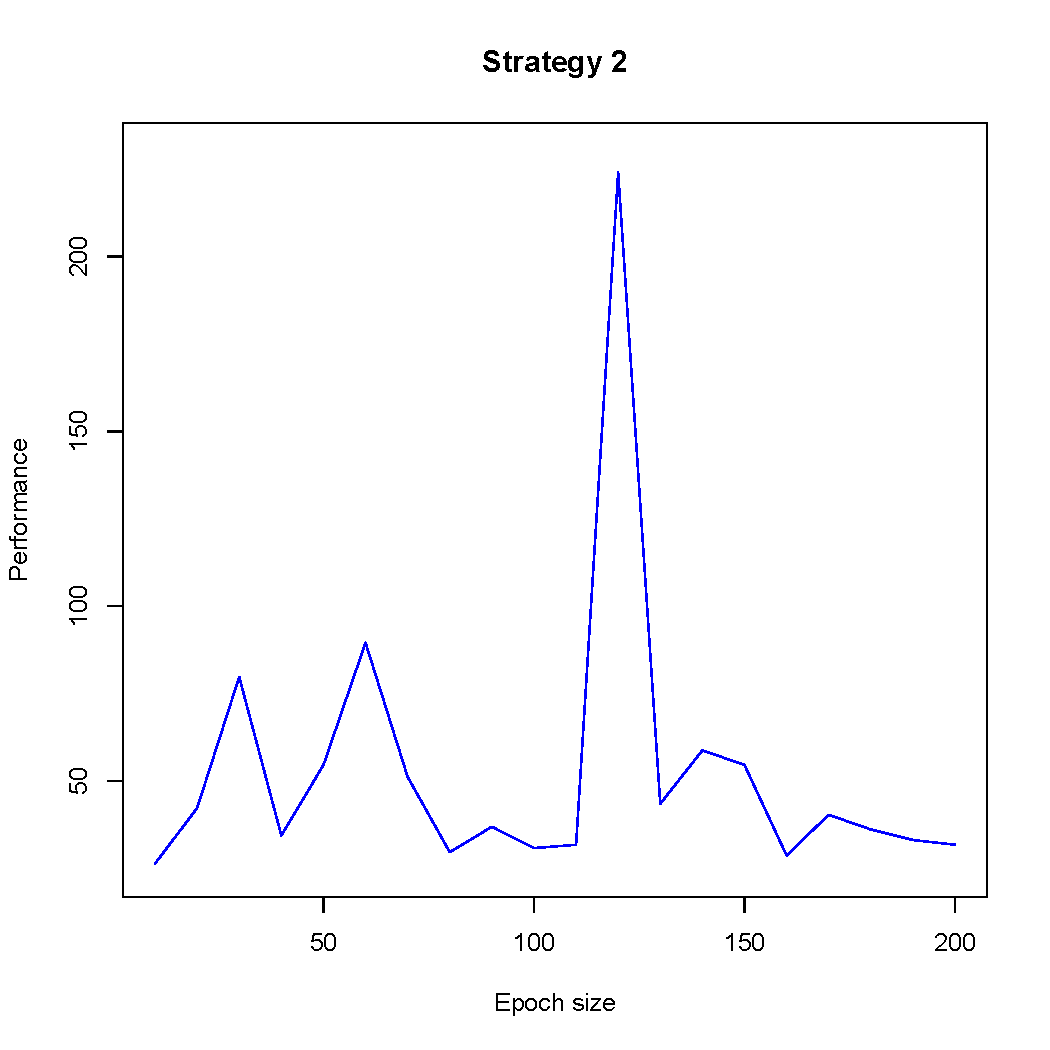
\includegraphics[width=0.4\textwidth]{graph2}
			 \end{center}
			 
			 Looking at the graphs, the first conclusion we had was that strategy $1$ was definitely better for our program than strategy $2$, the latter actually being very unstable, having a very high variation of average number of tuns. The performance of strategy $1$ seems to be related to the epoch size, since the performance changes somewhat significantly, although not in a particular trend, as the epoch size increases. It is good to note that that change in performance might be related to the randomness of the game, but in case the relation indeed exists, it seems that the optimal performance would occur for epoch size around $120$.\\
			 
			 While the average number of turns for strategy $1$ seems to be around $25$ to $30$, strategy $2$ has average performances ranging from as low as $26.34$ to as high as $224.16$. It is good to note, however, that the games with ridiculously large number of turns are anomalities caused by the strategy function chosen. Since the exploration probability decreases as the number of iterations increases, we have cases of games that last a long, long time. As an example, for $120$ epochs, we had a game that lasted $3783$ turns, which is far from ideal. That indicates that the strategy is probably not the best to take, since it proves to be very unstable depending on randomness. Besides, the average number of turns over epochs is around $60$ to $70$ epochs, which is far worse than for the simple and faster strategy $1$.\\
                
                \item % TODO: 4b
                \item % TODO: 4c
            \end{enumerate}                
    \end{enumerate}
\section*{Appendix}
\subsection*{Code for 2.c}
\begin{verbatim}
def T(a, s, s_prime):
  # takes an action a, current state s, and next state s_prime
  # returns the probability of transitioning to s_prime when taking action a in state s
  
  probability = 0.0

  # -2 -1 0 1 2
  for w in range(-2, 3):
    # hit the wedge (0)
    if abs(w) == 0:
      p_wedge = 0.4
    # hit region outside the wedge (-1 or 1)
    elif abs(w) == 1:
      p_wedge = 0.2
    # hit region outside of that (-2 or 2)
    else:
      p_wedge = 0.1

    # get the wedge and do % to loop around in case of going around circle
    wedge = (a.wedge + w) % throw.NUM_WEDGES

    # same thing, but now for the ring
    for r in range(-2, 3):
      # hit the ring
      if abs(r) == 0:
        p_ring = 0.4
      # hit region outside the ring
      elif abs(r) == 1:
        p_ring = 0.2
      # hit region outside of that
      else:
        p_ring = 0.1

      # get the ring and do % to loop around in case of going around circle
      ring = abs(a.ring + r)

      score = throw.location_to_score(throw.location(ring, wedge))
      if score == s - s_prime:
        probability += p_wedge * p_ring

  return probability
\end{verbatim}
\end{document}